\newgeometry{top=1cm, bottom=2cm}
\section{Vektorräume}
\begin{figure}[h!]
    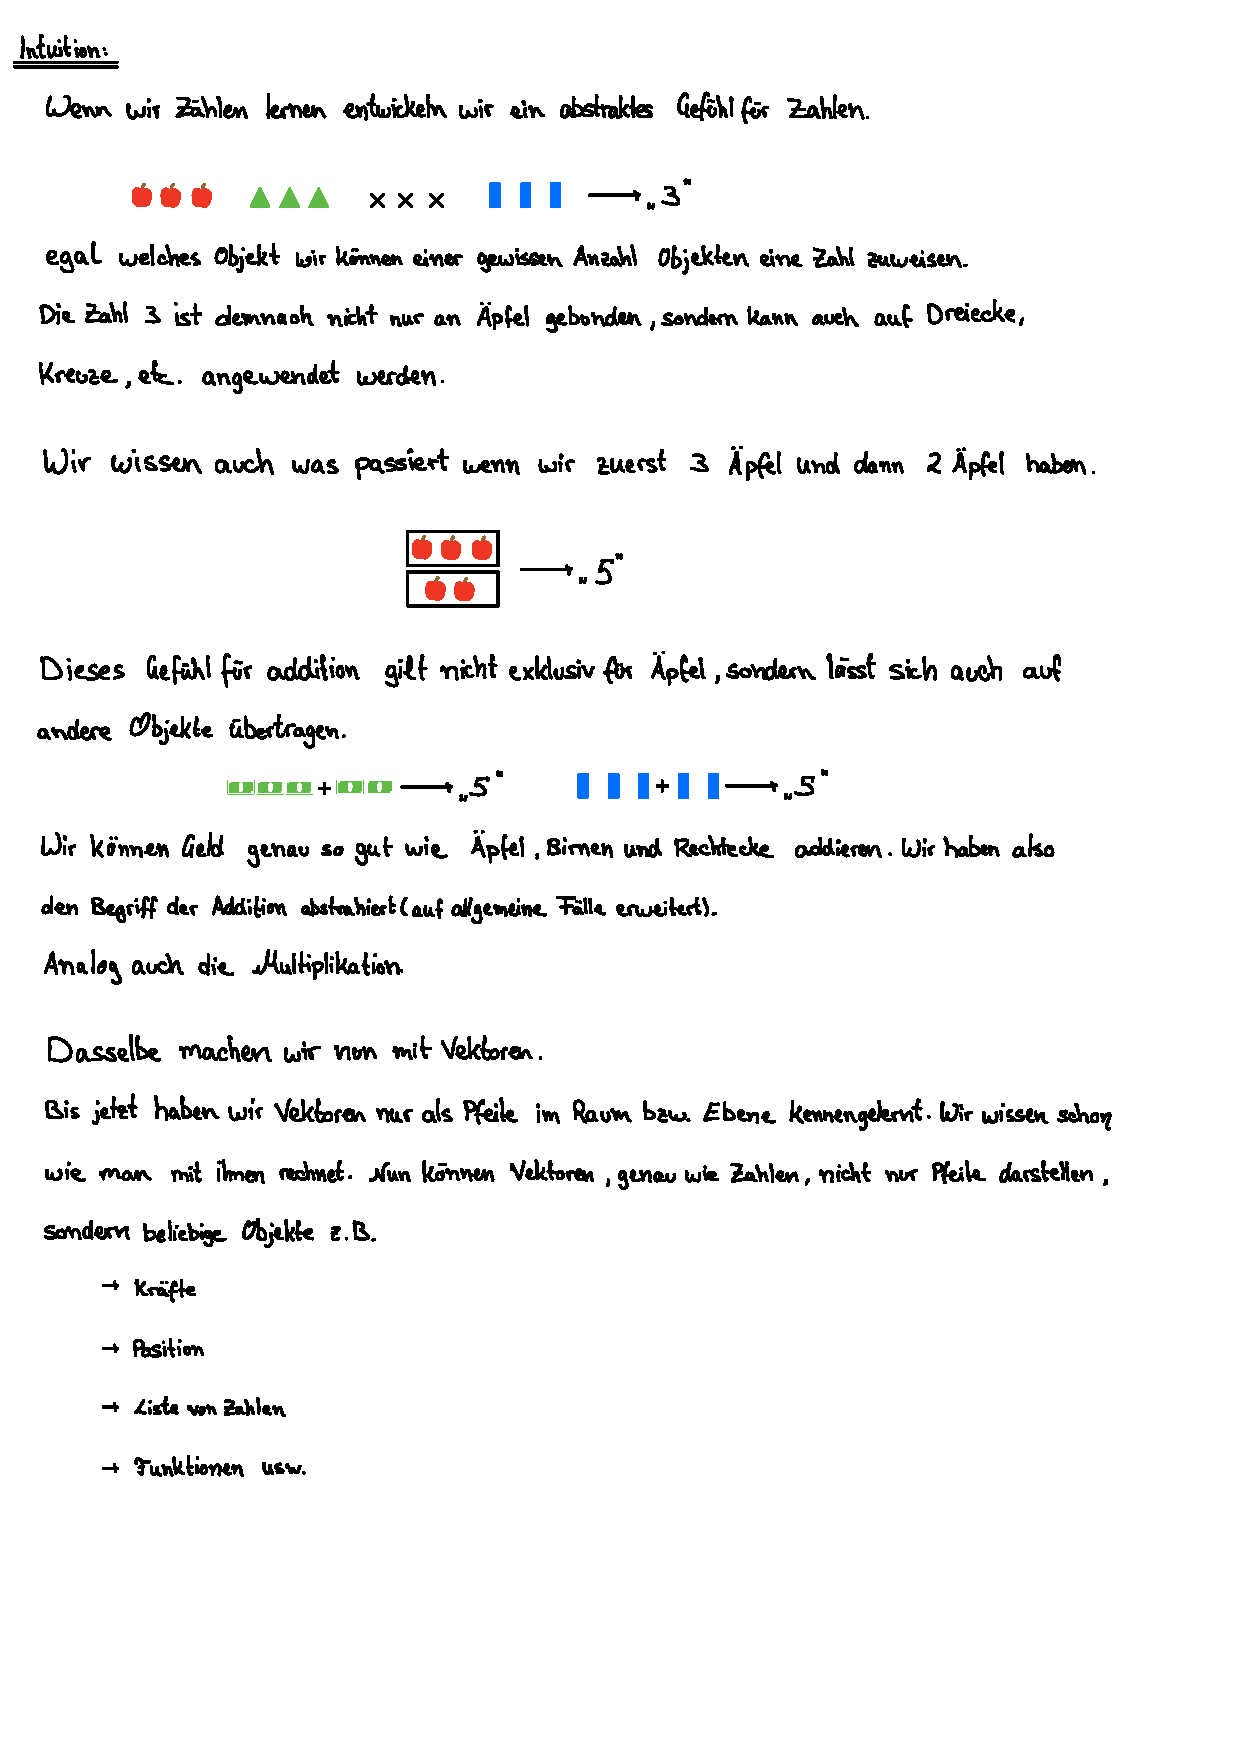
\includegraphics[page=1, scale=0.842]{pdf/04_Vektorraeume.pdf}
\end{figure}
\newpage
\includepdf[pages={2-}, 
            pagecommand={\thispagestyle{plain}}, 
            scale=0.95]{pdf/04_Vektorraeume.pdf}

\newgeometry{top=2.5cm, bottom=2cm}
\subsection{Beispielaufgaben} 
\vspace{1cm}
\subsubsection{} %Zardini S. 58
Seien
\[
v_1 = 
\begin{pmatrix}
1\\
0\\
2\\
\end{pmatrix}, v_2 =
\begin{pmatrix}
0\\
1\\
1\\
\end{pmatrix}, v_3=
\begin{pmatrix}
0\\
2\\
2\\
\end{pmatrix}, v_4=
\begin{pmatrix}
3\\
0\\
1\\
\end{pmatrix}
\]
Kann $w = \begin{pmatrix}
4\\
1\\
2\\
\end{pmatrix}$ als eine linear Kombination von $v_1,v_2,v_3,v_4$ beschrieben werden? Falls ja, geben Sie eine Linearkombination an. \\

\noindent \textbf{Lösung:}

\newpage
\subsubsection{} % Adi PVK Tag2
Es sei der Unterraum $U \subset \mathbb{R}^3$ gegeben durch 
\[
U := \{(x,y,z)^\top \in \mathbb{R}^3:x+y+z=0\}
\]
Bestimmen Sie eine Basis von $U$. \\

\noindent \textbf{Lösung:}
\vspace{7cm}

\subsubsection{} %Übung 14
Überprüfen Sie ob die folgenden Teilmengen Unterräume sind. Begründen Sie Ihre Antworten.
\begin{enumerate}[label=\alph*)]
    \item $\mathbb{R}^3 \subset \mathbb{R}^3$.
    \item $\{A\in \mathbb{C}^{n \times n}\: |\: A^\top = A \} \subset \mathbb{C}^{n \times n}$ für $n \in \mathbb{N}$.
    \item $\{p \in \mathcal{P}_3\: |\: p(1) = 0$ und $p(1100)=0\} \subset \mathcal{P}_3$, wobei $\mathcal{P}_n$ für $n \in \mathbb{N}$ der Vektorraum der Polynome mit Grad $\leq n$ ist.
    \item $\{(x_1, x_2, x_3)^\top \in \mathbb{R}^3 \: |\: \lvert x_1\rvert+\lvert x_2\rvert=\lvert x_3\rvert \}\subset \mathbb{R}^3$
\end{enumerate}

\noindent \textbf{Lösung:}

\newpage
\subsubsection{} %Adi PVK Tag 2
Betrachten Sie den Vektorraum $\mathcal{P}_3$ der reellen Polynome vom Grad $\leq$ 3 mit der Basis $\mathcal{B} = \{x^3+1,x^2+x-2,2x+1,x+2\}$.
\begin{enumerate}[label=\alph*)]
    \item Welches Polynom in $\mathcal{P}_3$ hat die Koordinaten $(2,1,-1,3)^\top$ bezüglich $\mathcal{B}$?
    \item Sei $p(x):=x^3+x^2+x+1$. Bestimmen Sie die Koordinaten von $p(x)$ bezüglich $\mathcal{B}$.
\end{enumerate}
\noindent \textbf{Lösung:}

\newpage
\subsubsection{} %Prüfung S12
Sei $V$ der von den Funktionen $\{1,x,x^2,e^x\}$ aufgespannte Vektrorraum mit dem Unterraum $U:=\{1,x,x^2\}$. Für zwei Funktionen $f,g \in V$ sei das folgende Skalarprodukt definiert:
\[
\langle f,g \rangle := f(0)g(0)+f'(0)g'(0)+f''(0)g''(0)+f'''(0)g'''(0).
\]\begin{enumerate}[label=\alph*)]
    \item Wie lautet die Norm von $f \in V$ bezüglich des gegebenen Skalarprodukts?
    \item Bestimmen Sie eine Orthonormalbasis in $U$ bezüglich des gegebenen Skalarprodukts.
    \item Verifizieren Sie, dass $\langle . \:,. \rangle$ tatsächlich ein Skalarprodukt ist.
\end{enumerate}

\noindent \textbf{Lösung:}

\newpage
\subsubsection{} %Zardini S.70
Sei folgendes Skalarprodukt auf $\mathcal{P}_4$ gegeben
\[
\langle p,q \rangle = \int_{0}^{1} p(x)q(x) \,dx.
\]
Finden Sie eine Orthonormalbasis für den Vektorraum $span(1,3x^4)$. \\

\noindent \textbf{Lösung:}
